\documentclass[conference]{IEEEtran}
\IEEEoverridecommandlockouts
% The preceding line is only needed to identify funding in the first footnote. If that is unneeded, please comment it out.
\usepackage{cite}
\usepackage{amsmath,amssymb,amsfonts}
\usepackage{algorithmic}
\usepackage{algorithm2e}
\usepackage{graphicx}
\usepackage{multicol}
\usepackage{textcomp}
\usepackage{xcolor}
\graphicspath{ {./images/} }
\SetKwComment{Comment}{/* }{ */}
\def\BibTeX{{\rm B\kern-.05em{\sc i\kern-.025em b}\kern-.08em
    T\kern-.1667em\lower.7ex\hbox{E}\kern-.125emX}}
\begin{document}

\title{Ring-Tossing Robot: Kinematic Trajectory Planning for Targeted Throwing of a Torus*\\
{\footnotesize \textsuperscript{*}Robotic Manipulation (6.4212, Fall 2024)}}
\author{\IEEEauthorblockN{Xin Zhang}
\IEEEauthorblockA{\textit{Dept. of EECS} \\
\textit{Massachusetts Institute of Technology}\\
Cambridge, MA \\
zhangx3@mit.edu}
}

\maketitle

\begin{abstract}
Throwing is a common action performed in our daily life, so it is interesting to explore how a robot may be programmed to throw objects toward given destinations. This paper describes the development of a system that commands a robot with a two-finger gripper to play the ring toss game in a simulation environment. I found a kinematic trajectory planning strategy that allowed the robot to throw a small object to a destination accurately. However, due to the lack of friction torque from the gripper fingers on the ring, the robot could not maintain an immobilizing grasp of the ring during the throwing action. Nevertheless, it still managed to let the ring land very close to the target peg.
\end{abstract}

\begin{IEEEkeywords}
robot, manipulation, torus, throw, simulator
\end{IEEEkeywords}

\section{Introduction}
Throwing is an interesting topic in robotic manipulation as it provides an efficient way to move an object to a destination potentially outside the kinematic range of the robot. Moreover, throwing is also an action performed in many games, and programming a robot to play such games can provide insight into different variants of the manipulation problem. In this project, I program a Kuka LBR iiwa robot with a Schunk WSG gripper to play the ring toss game in the Drake Simulator \cite{drake}.

I assume knowledge of the initial pose of the ring and that of the peg in the world frame. The system plans the kinematic trajectories to grasp the ring and throw it toward the peg. It then simulates the manipulation following the planned trajectories. I investigated different methods of planning the throwing trajectory. One strategy is to sample a position where the gripper should release the ring, compute the release velocity from there, and find a corresponding throwing trajectory. The other strategy is to let the gripper follow a predetermined segment of a circular path and attain the suitable release velocity at the end of the path. I tried kinematic trajectory optimization with both strategies, but the solver failed to find a solution within 28 attempts for the first strategy, and it produced suboptimal trajectories for the second strategy. Solving for a kinematic trajectory analytically along a fixed circular path produced the most consistent results that threw the ring close to the peg.

Although I managed to plan the trajectory for the robot to perform the throwing motion, due to limited friction torque between the gripper fingers and the ring, the gripper could not maintain a completely immobilizing grasp on the ring during the throwing trajectory. As a result, the ring could not land exactly over the peg. I explored potential solutions such as reducing the acceleration in the throwing trajectory, raising the gripper's force limit, modifying the model of the ring, and increasing the friction coefficients of the gripper and the ring. A smaller maximum acceleration, a stronger grasping force and an increased contact surface area between the gripper fingers and the ring partially alleviated the sliding problem. While unrealistically large friction coefficients could stop the sliding, they also prevented a smooth release of the ring. Similarly, adding a dent to the ring for grasping caused the ring to be stuck with gripper fingers at release time. Using a combination of the effective methods, the robot could let the ring land next to the peg, and I demonstrated the feasibility of the strategy for smaller objects by successfully throwing a small peg into a ring.

\section{Related Work}
Mason and Lynch \cite{mason1993dynamic} characterized dynamic manipulation as an operation that may consider forces inducing acceleration. They illustrated it by building a club-throwing robot and described different strategies for a robot to throw an object toward a target. In this project, I made the common assumption that the robot holds the ring in a completely immobilizing grasp until the gripper reaches the desired position and velocity to release it. Instead of building a robot dedicated to the throwing task, I used the model of an existing robot arm and a simple gripper.

Zeng et al. \cite{zeng2020tossingbot} and Liu et al. \cite{liu2022solution} used deep learning in tandem with a physics-based controller to throw arbitrary objects toward given destinations. In \cite{zeng2020tossingbot}, the grasping policies learned jointly with the throwing policies favored stable grasps which resulted in more consistent and accurate throwing despite different aerodynamics for different objects. Similarly, antipodal grasps are used in this project for their stability, but choosing a grasp for a ring requires additional consideration about its orientation relative to the peg when it reaches the end of the flying trajectory. Due to the time constraint for the project, I chose to neglect air resistance in the simulation.

The circular trajectory that Ramirez and Burgess \cite{ramirez2023robotic} used to simulate the throwing action in rock skipping inspired one of my strategies for planning the throwing trajectory. While they used kinematic trajectory optimization to find a corresponding trajectory for the robot joints, I found it preferable to compute a joint trajectory directly.

To my knowledge, there is no prior work on a robot playing the ring toss game. This project tackles the complexity that arises both from the ring toss game in general and from the limitations of using a robot model not customized for the game.

\section{Background}
\subsection{Problem Statement}
In the ring toss game, there is a fixed set of pegs, and the player tries to toss rings such that each ring lands over a peg. Without loss of generality, I simplify the game and simulate the scenario with a single peg and a single ring, and the goal is to let the robot grasp and throw the ring such that the ring lands over the peg.

\subsection{Projectile Motion}
Given the constrained space reachable by the gripper, the system needs to find a \textit{flying trajectory} that the ring may take from that space to the peg, and the robot must give the initial velocity of that flying trajectory to the ring when releasing it. For brevity, I call the trajectory followed by the ring during the throwing action the \textit{throwing trajectory}, and the corresponding trajectory for the robot's joints the \textit{generalized throwing trajectory}. Based on the assumption that the gripper has an immobilizing grasp of the ring during the throwing action, I also use ``throwing trajectory'' to refer to the gripper's trajectory when the context is unambiguous. I call the ring's position at the end of the throwing trajectory the \textit{release position}, and the velocity at that moment the \textit{release velocity}. The release position and the release velocity equal the initial position and the initial velocity of the flying trajectory respectively. In this section, I derive the initial velocity given the initial position and the goal position of the flying trajectory, noting that the flying trajectory is a trajectory of projectile motion.

Suppose we are in the world frame, and let $p_{init} \in \mathbb{R}^3$ be the position of the ring at the start of the flying trajectory, $p_{goal} \in \mathbb{R}^3$ be the position of the top of the peg where the flying trajectory ends. Let $T \in \mathbb{R}$ be the duration of the flying trajectory, $v_0 \in \mathbb{R}^3$ be the (translational) release velocity, $g \in \mathbb{R}^3$ be the gravitational acceleration.

The ring's velocity at time $t$ for $0 <= t <= T$ is
\begin{equation*}
v_0 + gT
\end{equation*}.

The constraints require
\begin{align*}
p_{goal} - p_{init} &= \int_{0}^{T} v_0 + g t \,dt \\
&= v_0 T + \frac{1}{2} g T^2
\end{align*}

Hence,
\begin{equation*}
v_0 = \frac{p_{goal} - p_{init}}{T} - \frac{1}{2} g T
\end{equation*}

If the direction of $v_0$ is unconstrained, we can choose a reasonable $T$ and compute the corresponding $v_0$.

In my second strategy where the throwing trajectory is along a segment of a circular path, the ring has a zero $z$-component in the velocity throughout the trajectory, and that determines $T$ so we do not need to make the choice there.
\begin{align*}
0 &= \frac{p_{goal}[2] - p_{init}[2]}{T} - \frac{1}{2} g[2] T \\
T &= \sqrt{\frac{2 (p_{goal}[2] - p_{init}[2])}{g[2]}}
\end{align*}

\subsection{From Constant Velocity to Constant Acceleration}
\label{const_acc}
In my implementation of the second strategy, I found it useful to first generate a constant-velocity generalized throwing trajectory $\text{Traj}_{cv}$ and then derive a constant-acceleration generalized throwing trajectory $\text{Traj}_{ca}$, such that both trajectories travel through the same path, have the same initial and final generalized positions, and reach the same final generalized velocity, but $\text{Traj}_{ca}$ has an initial generalized velocity of zero.

Given a trajectory $\text{Traj}$, I can evaluate the position at time $t$ as $\text{Traj}(t)$ for $0 <= t <= T$ where $T$ is the duration of $\text{Traj}$. Let $T_{cv}$ be the duration of $\text{Traj}_{cv}$ and $T_{ca}$ be the duration of $\text{Traj}_{ca}$. Let $v$ be the constant velocity in $\text{Traj}_{cv}$ and $a$ be the constant acceleration in $T_{ca}$. We require
\begin{align*}
\text{Traj}_{ca}(0) &= \text{Traj}_{cv}(0) \\
\text{Traj}_{ca}(T_{ca}) &= \text{Traj}_{cv}(T_{cv}) \\
a T_{ca} &= v \\
\end{align*}
From the equations above, we can deduce
\begin{align*}
&v T_{cv} = \frac{1}{2} a T_{ca}^2 \\
\Rightarrow\, &a T_{ca} T_{cv} = \frac{1}{2} a T_{ca}^2 \\
\Rightarrow\, &T_{ca} = 2 T_{cv} \\
\Rightarrow\, &a = \frac{v}{2 T_{cv}}
\end{align*}
For $0 <= t <= T_{ca} = 2 T_{cv}$,
\begin{align*}
\text{Traj}_{ca}(t) &= \text{Traj}_{ca}(0) + \frac{1}{2} a t^2 \\
&= \text{Traj}_{cv}(0) + \frac{1}{2} \frac{v}{2 T_{cv}} t^2 \\
&= \text{Traj}_{cv}(0) + \frac{t}{2 T_{cv}} \frac{v t}{2} \\
&= \text{Traj}_{cv}(0) + \frac{t}{2 T_{cv}} (\text{Traj}_{cv}(\frac{t}{2}) - \text{Traj}_{cv}(0))
\end{align*}
And now we have derived the constant-acceleration trajectory as a function mapping time to positions.

\section{Methodology}

\subsection{Simulation Setup}
Figure \ref{fig:scenario} shows the scenario of the experiments. The peg was modeled using a cylinder, and the ring was modeled using a torus. The ring is placed on a box for easier grasping. I chose the hydroelastic contact model for a more realistic contact simulation compared to the point contact model. The programs for the experiments were written in Python using the Drake toolbox \cite{drake}, and the models of the ring were created using Blender \cite{blender}.

\begin{figure}[ht]
\centering
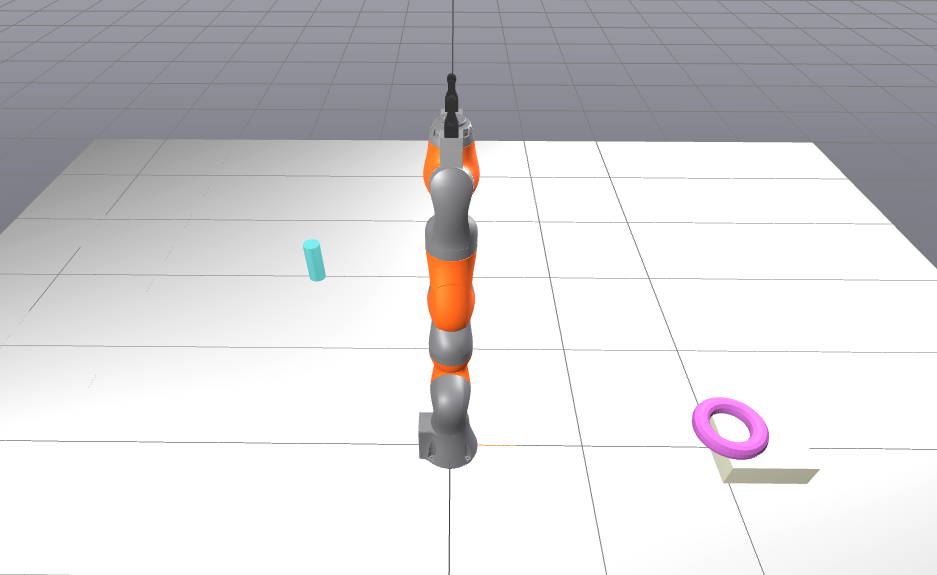
\includegraphics[width=0.45\textwidth]{images/scenario.png}
\caption{The scenario of the ring toss experiments in the simulator. The platform, the base of the robot arm and the cylinder are welded to the world.}
\label{fig:scenario}
\end{figure}

The default friction coefficient of the ring and that of the gripper fingers are both one. The ring has a mass of one gram, with a major radius of 10 cm and a minor radius of 3 cm. A preliminary experiment using a smaller ring with a minor radius of 2 cm encountered simulation problems where the gripper fingers penetrated through the ring during grasping, and I believe it was a manifestation of the difficulty in simulating contact with small objects.

\subsection{Manipulation workflow}

The manipulation can be divided into a few stages shown in Figure \ref{fig:manip_steps}. Given the initial poses of the peg and the ring, the system plans the trajectories for the different stages accordingly.

\begin{figure}[ht]
\centering
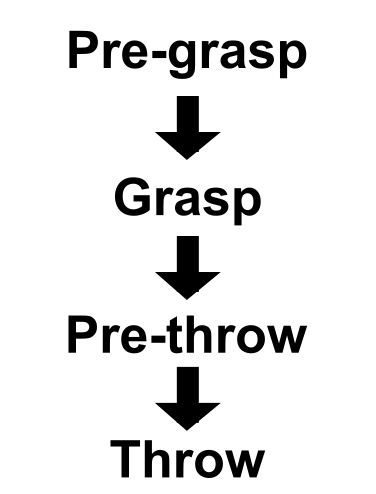
\includegraphics[width=0.1\textwidth]{images/manip_steps.png}
\caption{The manipulation workflow.}
\label{fig:manip_steps}
\end{figure}

In the pre-grasp phase, the gripper moves close to the ring without risking collisions. I manually specified the pre-grasping pose and the grasping pose of the gripper measured from the ring's frame. Then I use spatial algebra and inverse kinematics to find the corresponding generalized positions of the robot.

The size of the gripper fingers is small compared to the diameter of the ring. As a result, a rotation of the gripper after the grasping can require large contact forces to stabilize the ring again. To alleviate the problem, I leave sufficient time for the pre-throw stage where the robot slowly moves the ring to the start of the throwing trajectory and allows it to settle into that pose.

To plan the throwing trajectory, I investigated variations of two main strategies. The first one is to randomly sample a release position near the robot, relying on inverse kinematics to find the corresponding generalized trajectory. The second is to let the ring follow a predetermined segment of a circular path and attain the suitable release velocity at the end of the path. For both strategies, I tried kinematic trajectory optimization as well as more analytical methods of generating a corresponding generalized throwing trajectory. To release the ring, the gripper fingers open at the end of the generalized throwing trajectory. Details of the different strategies and their performance are described in Section \ref{results}.

\subsection{Grasp selection}
Antipodal grasps are chosen for their stability, but choosing a grasp for a ring is particularly interesting because the center of mass of the ring cannot lie between the contact points as shown in Figure \ref{fig:center_of_mass}, and the orientation of the ring matters as the ring may miss the peg in some orientations as illustrated in Figure \ref{fig:swing}.

\begin{figure}[ht]
\centering
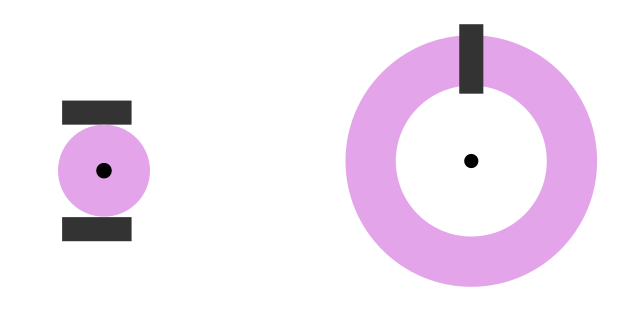
\includegraphics[width=0.2\textwidth]{images/center_of_mass.png}
\caption{The gripper cannot grasp the ring (right) such that the center of mass of the ring lies between the contact points of the grasp, like how it may grasp a small ball (left). The black dots represent the centers of mass, and the rectangles represent the fingers of the gripper.}
\label{fig:center_of_mass}
\end{figure}

\begin{figure}[ht]
\centering
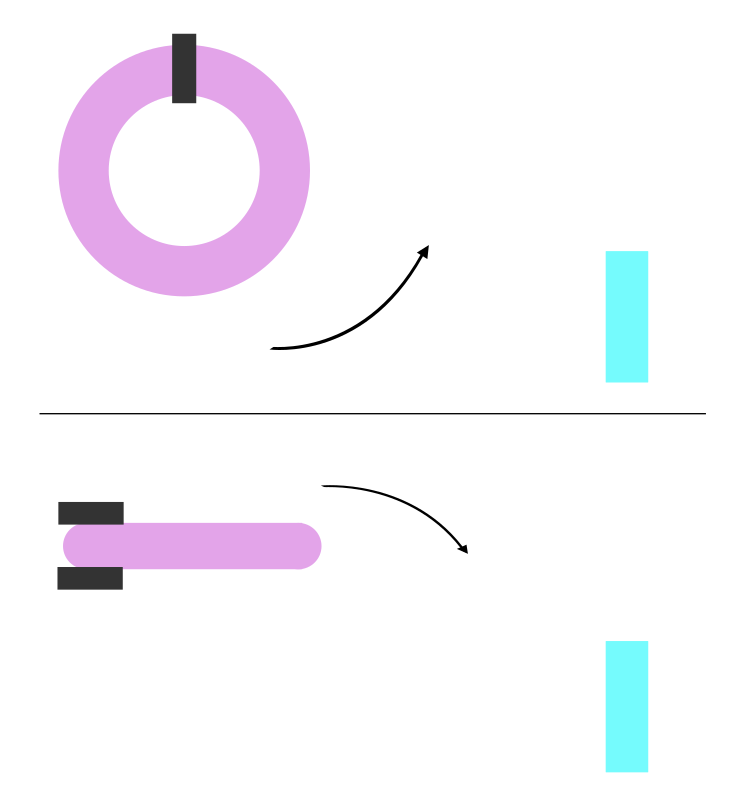
\includegraphics[width=0.2\textwidth]{images/swing.png}
\caption{Unlike how the robot in \cite{zeng2020tossingbot} may grasp a screwdriver and swing it like a pendulum before throwing it into a box, the robot in our system cannot swing the ring towards the peg in an orientation that prevents it from landing over the peg (top). The bottom diagram shows one feasible orientation of the ring upon release.}
\label{fig:swing}
\end{figure}

Given a desired release velocity, Figure \ref{fig:grasp_direction} shows two corresponding grasps that help prevent the gripper from blocking the flying trajectory.
\begin{figure}[ht]
\centering
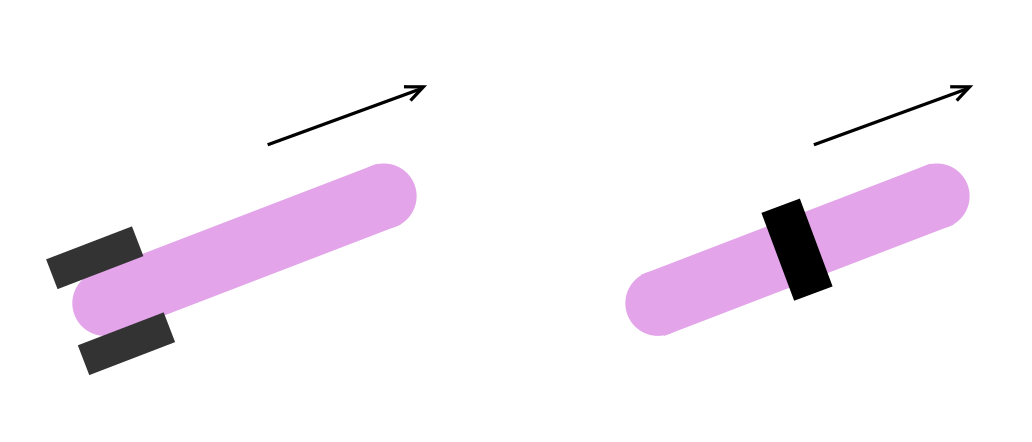
\includegraphics[width=0.3\textwidth]{grasp_direction.png}
\caption{Two choices of the grasp pose at release time given the direction of the release velocity indicated by the arrows.}
\label{fig:grasp_direction}
\end{figure}


\section{Results and Discussion}
\label{results}
The objective of the task implies a straightforward performance evaluation criterion. The goal is to let the ring land as close to the peg as possible at the end of the flying trajectory, using Euclidean distance as the metric. The performance depends primarily on the planning and the execution of the throwing trajectory after the gripper has successfully grasped the ring, and that is the focus of this section.

\subsection{Validating the Computation}
Given a randomly sampled release position $p_r$, I validated the computation of the release velocity $v_r$ by setting the ring's initial position to be $p_r$ and its initial velocity to be $v_r$ at the beginning of the simulation. The ring successfully landed over the peg in multiple experiments with different release positions.

\subsection{Sampling-based Planning of the Throwing Trajectory}
My first attempt at trajectory planning was to express it as a kinematic trajectory optimization problem. I would like to include the position constraints on the gripper based on the release position, and there are infinitely many release positions reachable by the gripper. Since Drake's \texttt{AddPositionConstraint} function does not take decision variables as the position bounds, I formulated the optimization problem with a release position sampled randomly from a uniform distribution near the robot. Moreover, the release velocity should be incorporated into the constraints too, but Drake's \texttt{KinematicTrajectoryOptimization} interface only provides a constraint on generalized velocity. Hence, I used differential inverse kinematics to find a generalized release velocity $u_r$ that can be used with the interface. To generate an initial guess for the optimization problem solver, a ``pre-release'' position is computed from the release position and the release velocity that the gripper should pass through just before releasing the ring, and inverse kinematics is used to find generalized positions for both the release pose and the pre-release pose of the gripper. We can then extrapolate from the two generalized positions to obtain a joint throwing trajectory. Algorithm \ref{alg:sample_opt} shows the pseudocode for the algorithm. The notation $\epsilon$ denotes a small positive real number, and different occurrences of $\epsilon$ in the pseudocode may represent different values. We denote the forward kinematics function by \textit{FK}, the inverse kinematics function by \textit{IK}, the differential inverse kinematics function by \textit{DiffIK}, the kinematic trajectory optimization instance constructor by \textit{KinTrajOpt}, and let $k \geq 1$ be a positive real constant. The \textit{initial\_velocity} function computes the release velocity of the ring, and \textit{gripper\_release\_pose} computes the gripper's pose at release time.

\begin{algorithm}
\caption{The algorithm for sampling-based throwing trajectory planning with kinematic trajectory optimization}\label{alg:sample_opt}
\KwData{$^{W}X^{ring}$, $^{W}X^{peg}$, $^{ring}X^{gripper}$, $max\_tries$}
$tries \gets 0$\;
\While{$tries < max\_tries$}{
$p_r \gets$ sample\_release\_position()\;
$v_r \gets$ initial\_velocity($^{W}X^{peg}$, $p_r$)\;
$X_r \gets$ gripper\_release\_pose($p_r$, $v_r$, $^{ring}X^{gripper}$)\;
\If{$q_r \gets \text{IK}(X_r)$ fails}
{continue\;}
$p_r' \gets p_r - 0.01 \times v_r$ \Comment*[r]{pre-release}
$X_r' \gets$ gripper\_release\_pose($p_r'$, $v_r$, $^{ring}X^{gripper}$)\;
\If{$q_r' \gets \text{IK}(X_r')$ fails}
{continue\;}
$q_0 = q_r - k (q_r - q_r')$\;
$X_0 = \text{FK}(q_0)$
\Comment*[r]{beginning of the throwing trajectory}
$u_r = \text{DiffIK}(q_r, v_r)$\;
$opt = \text{KinTrajOpt}()$\;
$opt.\text{AddDurationCost()}$\;
$opt.\text{AddPathLengthCost()}$\;
$opt.\text{AddConstraint}(X_0 - \epsilon \leq$ initial pose $\leq X_0 + \epsilon)$\;
$opt.\text{AddConstraint}(X_r - \epsilon \leq$ final pose $\leq X_r + \epsilon)$\;
$opt.\text{AddConstraint}((q_r, u_r) - \epsilon \leq$ (final generalized positions, final generalized velocity) $\leq (q_r, u_r) + \epsilon)$\;
$opt.\text{AddConstraint}($position, velocity and acceleration bounds from the robot configuration)\;
$traj_{guess} \gets$ interpolate between $q_0$ and $q_r$ with a duration of $0.01 \times k$\;
$opt.\text{SetInitialGuess}(traj_{guess})$\;
\If{$traj \gets opt.\text{Solve}()$ succeeds}
{\Return $traj$}
$tries \gets tries + 1$\;
}
\end{algorithm}

The algorithm failed to return a trajectory after 28 attempts at kinematic trajectory optimization. The final velocity constraint is the primary source of difficulty in the optimization problem, as the algorithm successfully returned a trajectory without that constraint. However, the resulting trajectory could not provide the desired release velocity.

I then tried removing the trajectory optimization part of the algorithm and instead used the initial guess as the actual generalized throwing trajectory. However, the resulting trajectories often had undesirable rotations that flipped the ring, causing it to hit the fingers upon release, as shown in Figure \ref{fig:sample_rotation_traj}. Reducing $k$ could give a shorter trajectory with less ring-flipping rotation, but in the cases where the ring was released smoothly, it still missed the target, likely due to the lack of time to accelerate to the desired release velocity.

\begin{figure}[ht]
\centering
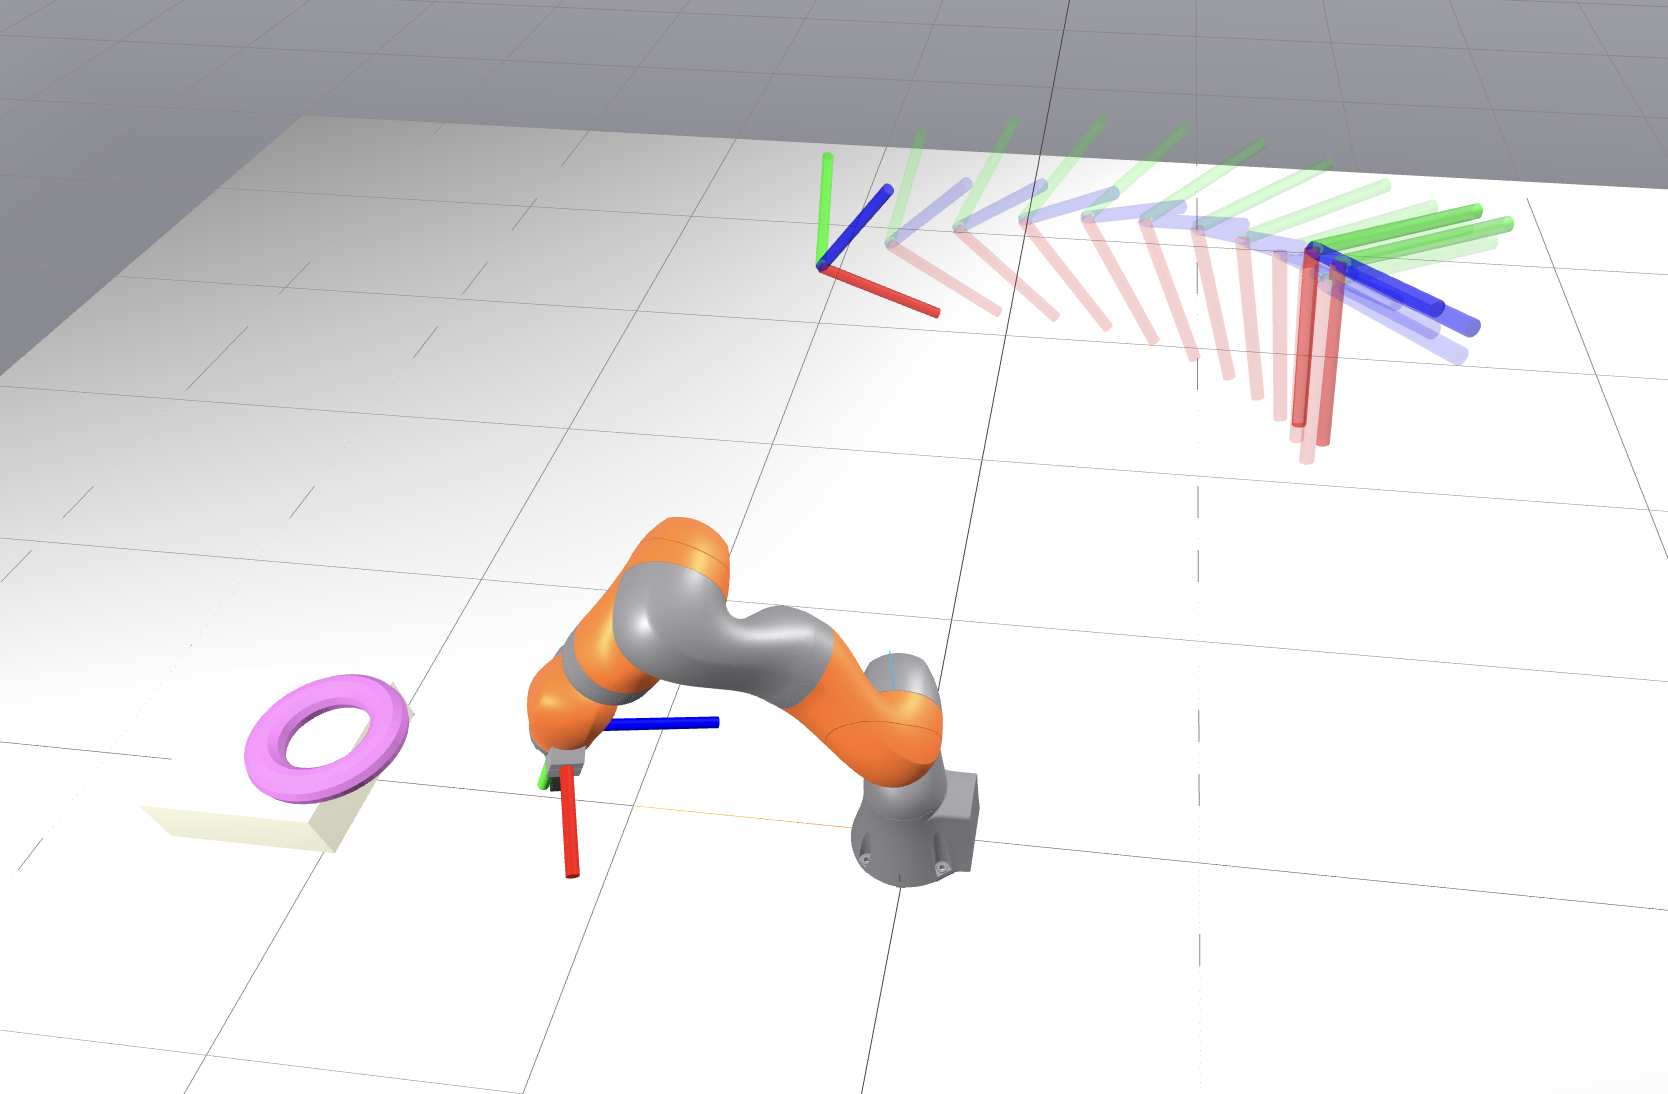
\includegraphics[width=0.45\textwidth]{images/sample_rotation_traj.png}
\caption{A gripper throwing trajectory (from left to right) generated by the sampling-based strategy with extrapolation from the generalized release position and the generalized pre-release positions. We can observe rotations along the trajectory that flips the ring.}
\label{fig:sample_rotation_traj}
\end{figure}

\subsection{Planning a Throwing Trajectory along a Fixed Path}
Inspired by the throwing trajectory used in \cite{ramirez2023robotic}, I simplified the trajectory planning problem by restricting the throwing trajectory to move along a predetermined circle, as shown in Figure \ref{fig:circle}. For simplicity, we assume the angle $\Delta$ is negligible, i.e., the path traveled by the gripper coincides with the path traveled by the ring. Such a path can be generated by changing the position of a single revolute joint of the robot arm, so every gripper pose along the trajectory is achievable by at least one generalized position of the robot. That joint's position $\theta$ equals the angular displacement of the gripper from the default position with respect to the center of the circular path. This approach is still able to give a release velocity in arbitrary directions in the $xy$-plane of the world frame, and the gripper just needs to release the ring at a point on the circle where the tangent meets the peg's position in the $xy$-plane, as indicated by the arrow in Figure \ref{fig:circle}.

\begin{figure}[ht]
\centering
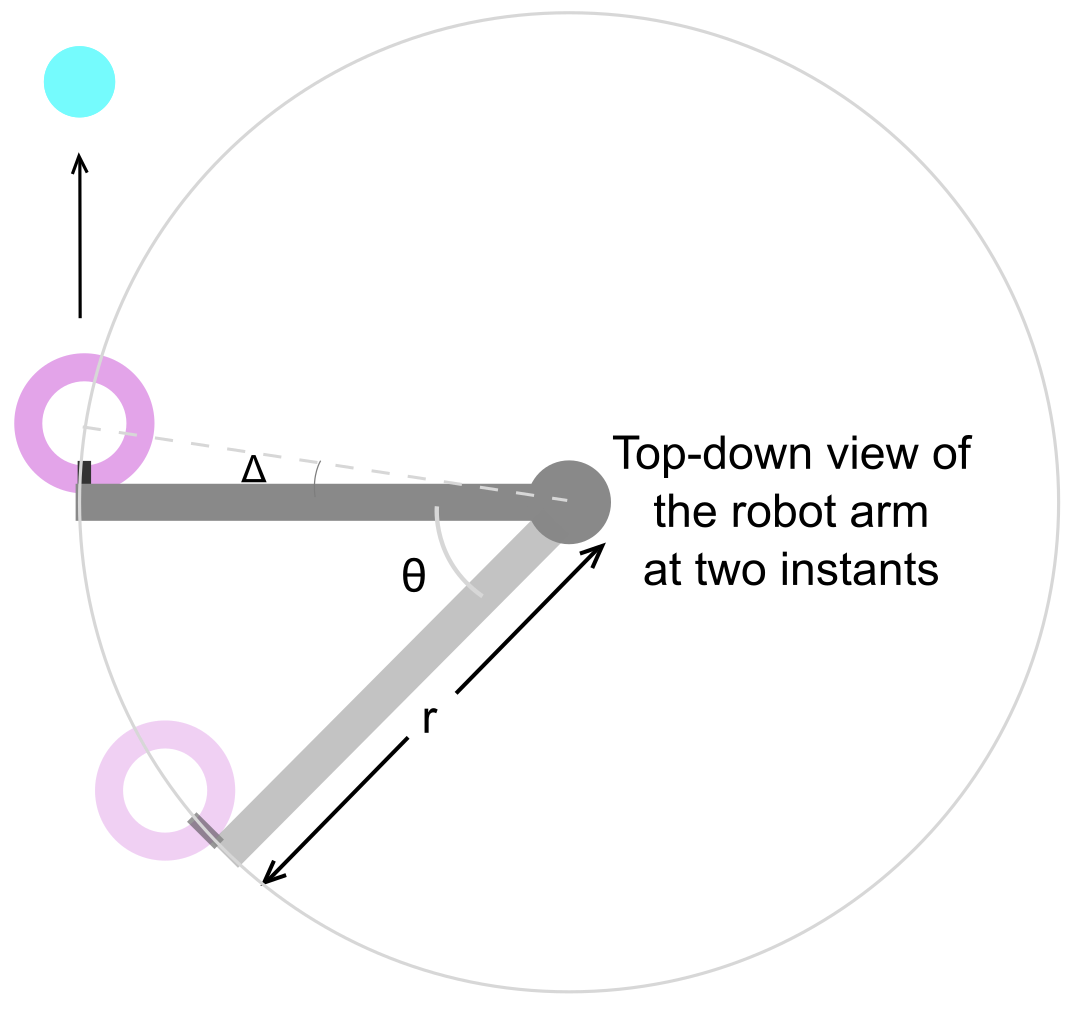
\includegraphics[width=0.45\textwidth]{images/circle.png}
\caption{A top-down view of the circular path along which the gripper travels. The blue disk is the top-down view of the peg, and the arrow indicates the direction in which the ring would travel if released at the leftmost point of the path.}
\label{fig:circle}
\end{figure}

I first tried using kinematic trajectory optimization to find a generalized throwing trajectory with the desired release velocity. I generated a joint trajectory by changing the joint position $\theta$ at some arbitrary constant speed, ending at the position where the ring should be released. The resulting trajectory is used as an initial guess for the optimization problem solver. Using the initial and the final gripper pose constraints and the release velocity constraint, I formulated a kinematic trajectory optimization problem similar to that described in Algorithm \ref{alg:sample_opt}. However, Figure \ref{fig:circle_rotation_traj} shows that the resulting trajectories have undesirable rotations near the points where the gripper pose is constrained. Adding a pose constraint in the middle of the trajectory did not reduce the rotations, and the solver failed to return a solution after I added a pose constraint very close to the end of the trajectory.

\begin{figure}[ht]
\centering
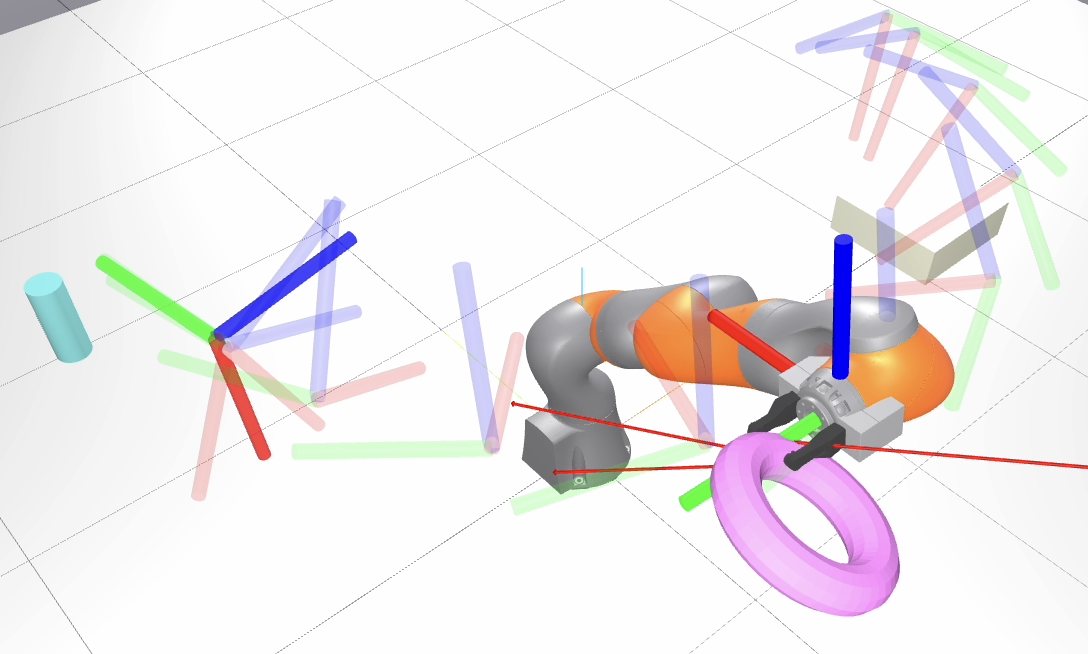
\includegraphics[width=0.45\textwidth]{images/circle_rotation_traj.png}
\caption{A gripper throwing trajectory (from right to left) generated by kinematic trajectory optimization based on an initial guess along a segment of the circular path. We can observe rotations along the trajectory that flips the ring.}
\label{fig:circle_rotation_traj}
\end{figure}

Since I was already generating a constant-velocity generalized throwing trajectory,  I decided that it was not necessary to use kinematic trajectory optimization to find a trajectory satisfying the constraints. Let $r$ be the radius of the circular path, and for the desired release speed $|v|$, the angular speed $| \dot{\theta} |$ should satisfy $r |\dot{\theta}| = |v|$ at release time. A naive generalized throwing trajectory $\text{Traj}_{cv}$ has a constant speed of $|\dot{\theta}|$, and such a trajectory is easy to generate through interpolation. However, the gripper brings the ring to the start of the throwing trajectory and stops there for the ring to stabilize in the pre-throw stage. The instantaneous transition from stationary to a non-zero speed causes a large acceleration which makes the ring slide quickly away from the gripper. Choosing a grasp that pushed the ring along the throwing trajectory slightly reduced the sliding as shown in Figure \ref{fig:forward_onward}. I further addressed the sliding problem by deriving a constant-acceleration generalized throwing trajectory from $\text{Traj}_{cv}$ using the method described in Section \ref{const_acc}, such that the resulting trajectory started with zero speed and ends with $|\dot{\theta}|$ after the same total displacement as the $\text{Traj}_{cv}$, attaining the same release position and release velocity for the ring.

\begin{figure}[ht]
\centering
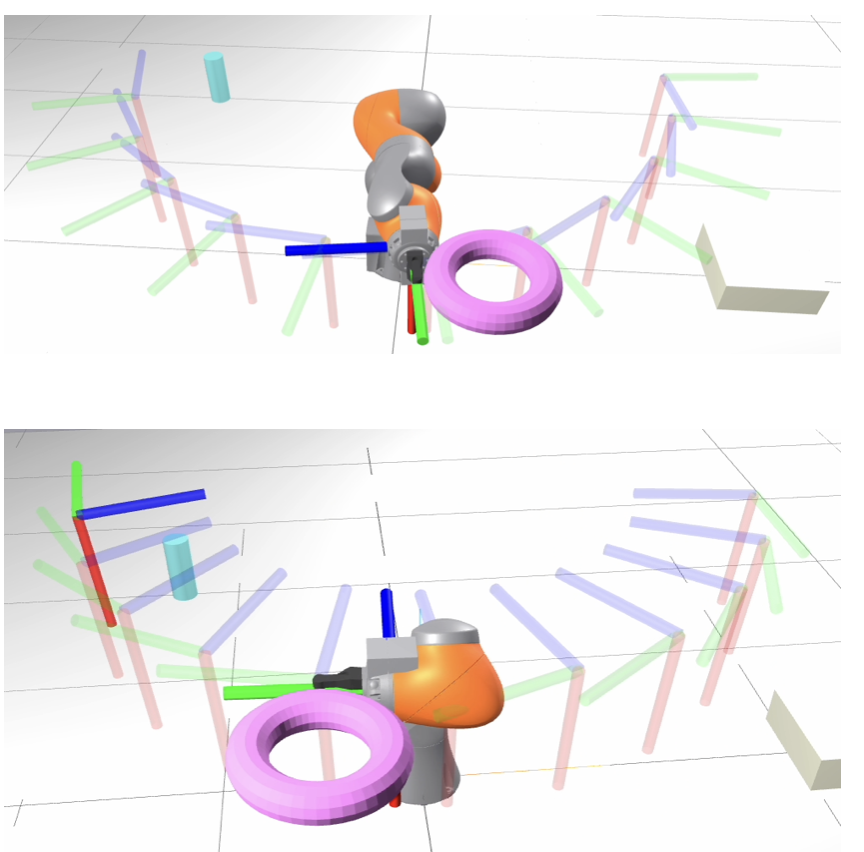
\includegraphics[width=0.45\textwidth]{images/forward_onward.png}
\caption{With the same angular velocity with respect to the center of the circular path, pushing the ring with the gripper (bottom) allowed the ring to remain in the grasp for slightly longer than slinging it (top) before the ring slid out of the grasp.}
\label{fig:forward_onward}
\end{figure}

The smaller maximum acceleration of the ring allowed it to remain in the grasp for much longer, but the sliding still caused the ring to deviate from the precomputed throwing trajectory. I tried increasing the contact force from the gripper fingers and changing the model of the ring to flatten its top and bottom, thereby increasing the area of contact with the gripper fingers. With a further decrease in the acceleration by utilizing the entire range of motion of the rotating joint, that gave the best throw among all the experiments, as shown in Figure \ref{fig:full_circle}.

\begin{figure}[ht]
\centering
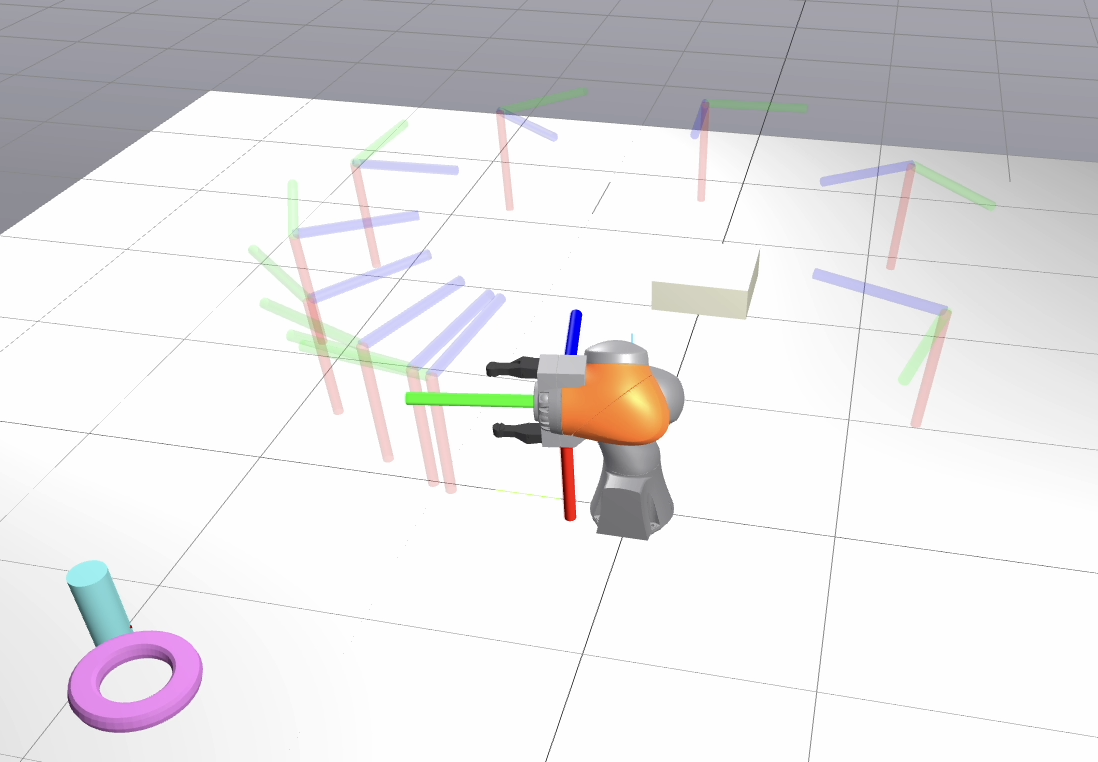
\includegraphics[width=0.45\textwidth]{images/full_circle.png}
\caption{Throwing a ring with flat top and bottom at constant joint acceleration through a full circle. The ring landed next to the peg.}
\label{fig:full_circle}
\end{figure}

I tried adding a dent to the ring to stop the sliding, but the large force exerted by the fingers in the throwing trajectory caused them to get stuck in the dent when it was time to release the ring. I also tried increasing the friction coefficients of both the ring and the gripper fingers, but the coefficients sufficient to stop the sliding were unrealistically large, and the friction also made the ring stop with the fingers when it was released.

Although the system could not throw the ring precisely over the peg, I demonstrated the feasibility of the analytical trajectory planning approach by playing the inverted ring toss game - the robot threw a small peg towards a ring instead. The peg successfully landed at the ring's position as shown in Figure \ref{fig:throw_peg}. The task succeeded with multiple different ring positions.

\begin{figure}[ht]
\centering
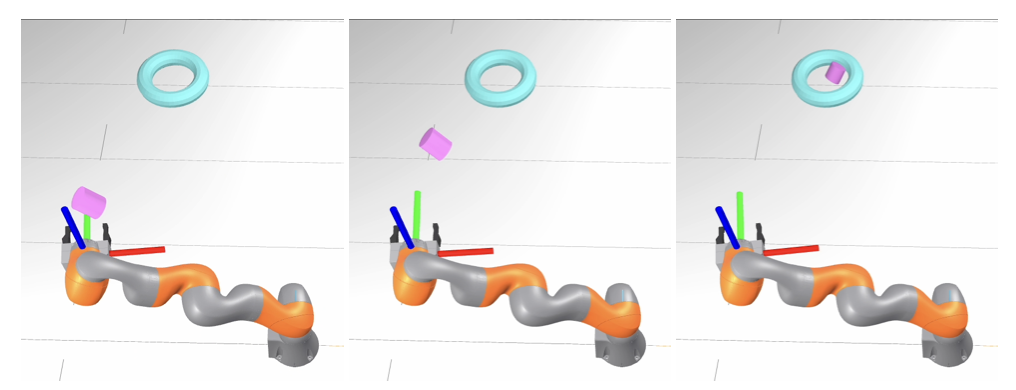
\includegraphics[width=0.45\textwidth]{images/throw_peg.png}
\caption{Throwing a peg into a ring with a constant joint acceleration moving the gripper along a circular path.}
\label{fig:throw_peg}
\end{figure}

\section{Conclusion and Future Work}
In this project, I programmed a robot with a simple gripper to play the ring toss game. The system successfully planned and executed the grasping and throwing trajectories to throw an object toward a target position. However, the ring slid during the throwing trajectory due to the lack of friction torque from the gripper fingers, violating the assumption of an immobilizing grasp in the trajectory. Nevertheless, by reducing the acceleration in the throwing trajectory and increasing the contact area between the fingers and the ring, I significantly alleviated the problem and managed to let the ring land very close to the peg.

My investigation in the trajectory planning revealed that kinematic trajectory optimization is not suitable for problems that impose strict constraints on the exact pose and velocity at which the object must be thrown. The analytical approach for finding a joint trajectory yielded much more controllable results.

Future work may explore the use of a robot with wider fingers or a more complex hand to exert sufficient torque on the ring for an immobilizing grasp throughout the throwing trajectory. Alternatively, it is also plausible to lift the assumption of an immobilizing grasp, calculate the condition for the ring to slide out of the grasp, and release the ring via the sliding motion.

\section{Acknowledgements}
I would like to express my gratitude towards Professor Tomas Lozano-Perez and the teaching assistants (Quincy Johnson, Nicholas Pfaff, Ethan Yang, Shruti Garg and Ryan Yang) for their guidance throughout the course.

\bibliographystyle{plain}
\bibliography{refs}
\end{document}
